\documentclass{beamer}
\usepackage{listings}
\usepackage{multicol}
\usepackage[ruled,vlined]{algorithm2e} 
\usepackage{algpseudocode}


\lstset{
%language=C,
frame=single, 
breaklines=true,
columns=fullflexible
}
\graphicspath{./figures/}
\usepackage{subcaption}
\usepackage{url}
\usepackage{tikz}
\usepackage{tkz-euclide} % loads  TikZ and tkz-base
%\usetkzobj{all}
\usetikzlibrary{calc,math}
\usepackage{float}
\newcommand\norm[1]{\left\lVert#1\right\rVert}
\renewcommand{\vec}[1]{\mathbf{#1}}
\usepackage[export]{adjustbox}
\usepackage[utf8]{inputenc}
\usepackage{amsmath}
\providecommand{\pr}[1]{\ensuremath{\Pr\left(#1\right)}}
\providecommand{\brak}[1]{\ensuremath{\left(#1\right)}}
\providecommand{\cbrak}[1]{\ensuremath{\left\{#1\right\}}}
\providecommand{\sbrak}[1]{\ensuremath{\left[#1\right]}}
\usetheme{Boadilla}

\SetKwInput{KwInput}{Input}                % Set the Input
\SetKwInput{KwOutput}{Output}              % set the Output



\title{Research Paper Presentation}
\author{MANNAM SARANDEEP-CS20BTECH11030}
\institute{INDIAN INSTITUTE OF TECHNOLOGY,HYDERABAD}
\date{\today}
\begin{document}

\begin{frame}
\titlepage
\end{frame}

\begin{frame}{\textbf{Title and Author}}
    \begin{block}{Title}
    Performance comparison of DTX detection schemes
    for 5G NR PUCCH
    \end{block}
    
    \begin{block}{Author}
    \begin{enumerate}
        \item Young-Hoon Kim
        \item Hyungsik Ju
        \item Chan Bok Jeong
        \item Moon-Sik Lee
    \end{enumerate}
    Future Mobile Communication Research Division
Electronics and Telecommunications Research Institutes
Daejeon, South Korea
    \end{block}
\end{frame}

\begin{frame}{\textbf{Abstract}}
    \begin{itemize}
    \item  The detection of discontinuous transmission (DTX) at the receiver
    \item  Demodulation of the uplink control information (UCI) that is transmitted on the 5G New Radio (NR) Physical Uplink Control Channel (PUCCH)
    \item Two feasible detection schemes of the DTX for 5G NR PUCCH format 0 are considered.
    \item The performance comparisons of
     these are carried out by the computer simulations under several situations.
     \item  The simulation results show that these meet the performance metrics described in the 3GPP standards.
    \end{itemize}
\end{frame}
\begin{frame}{\textbf{Keywords}}
    \begin{block}{DTX}
    Discontinuous transmission (DTX) is a method of momentarily powering-down a mobile or portable wireless telephone set when there is no voice input .This optimizes the overall efficiency of a wireless voice communication system.
    \end{block}
    \begin{block}{Physical uplink control channel(PUCCH)}
     PUCCH is an uplink physical channel that carries UCI (Uplink Control Information).UCI consists of HARQ (Hybrid Automatic Repeat Request) feedback, CSI (Channel State Information) and SR (Scheduling Request).
    \end{block}
    \begin{block}{PUCCH Format}
    Depending on what kind of information the UCI in PUCCH contains, PUCCH is classified into various formats.
    \end{block}
\end{frame}
\begin{frame}{Keywords}
\begin{block}{UE}
A device carries the uplink control information (UCI) on the Physical Uplink Control Channel (PUCCH).
\end{block}
\begin{block}{TX and RX}
TX and RX are abbreviations for Transmit and Receive, respectively.
\end{block}
\begin{block}{gNB}
The gNB is a 3GPP 5G Next Generation base station which supports the 5G New Radio.
\end{block}
\begin{block}{SNR}
The Signal to noise ratio(SNR) is the difference between the received wireless signal and the noise floor.
\end{block}
    
\end{frame}
\begin{frame}{\textbf{Introduction}}
\begin{itemize}
   \item 5G NR (New radio) is latest cellular wireless technology which follows 3GPP specifications.
    \item UCI can be transmitted on PUCCH using five different formats for various situations and scenarios 
    \item  Short-PUCCH such as format 0 and
    format 2 can be transmitted in short-duration (1 or 2 OFDM symbols).
    \item On the other hand, long-PUCCH such as format
    1,3 and 4 can be transmitted occupying from 4 to 14 OFDM symbols.
    \end{itemize}
    \end{frame}
\begin{frame}{\textbf{Introduction}}
\begin{itemize}
    \item  Whenever the number of bits of UCI is
less than equal to 2, format 0 and 1 should be used to carry only HARQ and Scheduling Request (SR). The other formats can be used to transmit UCI more than 2 bits for carrying CSI.
    \item In this paper, we focus only on the detection of 5G NR PUCCH format 0 that is quite different from the other formats.
    \end{itemize}
    
\end{frame}
     
    

    

\begin{frame}{\textbf{Introduction}}
    \begin{figure}
        \centering
        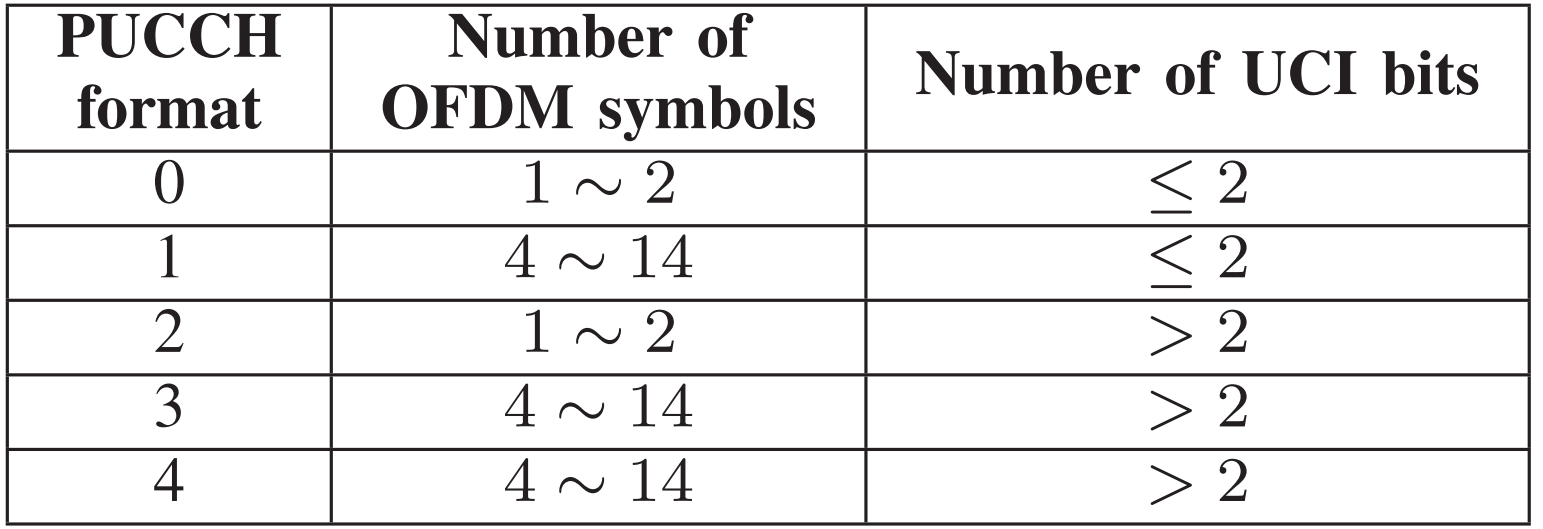
\includegraphics[scale=0.3     
        ]{TABLE_PUCCH_FORMATS.png}
        \caption{Table regarding 5G PUCCH formats}
    \end{figure}    
\end{frame}


\begin{frame}{\textbf{System Description}}
    \begin{figure}
        \centering
        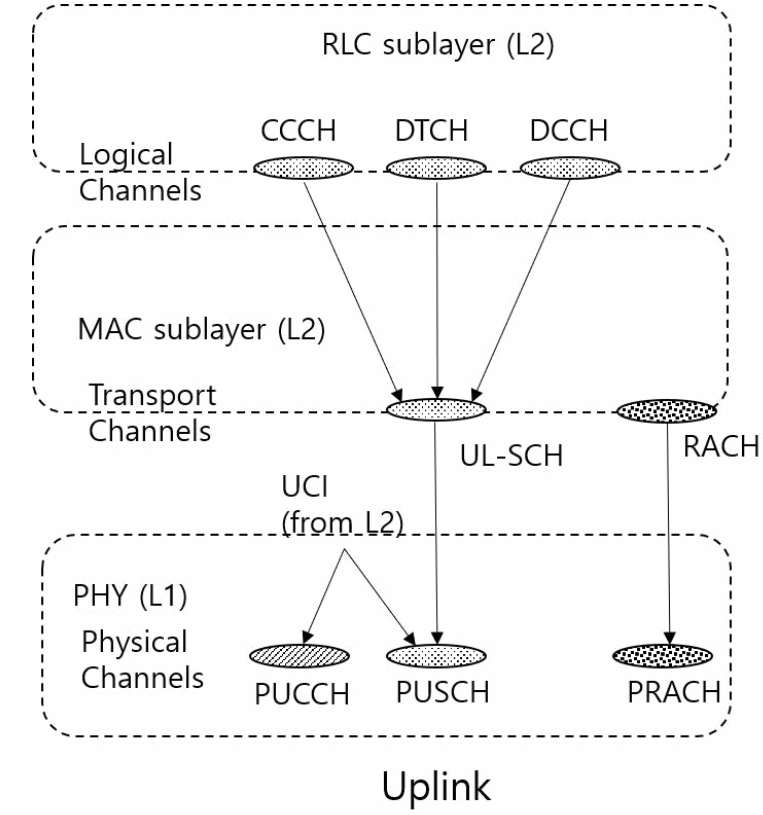
\includegraphics[scale=0.3     
        ]{UPLINK.png}
        \caption{ Mapping between UL channels}
    \end{figure} 
\end{frame}

\begin{frame}{\textbf{System Description}}
    \begin{itemize}
        \item A PUCCH format for a UE can configured done by the Radio Resource Control (RRC) signaling from gNB (Next generation nodeB).
        \item  The resource configuration for the UE
PUCCH format can be defined by several RRC parameters
such as intraSlot Frequency Hopping, starting PRB, second Hop-PRB, no of Symbols, and starting Symbol Index.
        \item  A PUCCH format 0 can be used during RRC connection, because the UE has only HARQ-ACK information bit and can be used under the
situation when the low latency is needed.
 \end{itemize}
\end{frame}
\begin{frame}{System Description}
    \begin{itemize}
        \item PUCCH format 0 sequence is generated according to
        \begin{align}
            x(l.N^{RB}_{sc}+n)=r^{(\alpha,\delta)}_{u,v}(n)
        \end{align}
$n=0,1,2,...N^{RB}_{sc}-1$
\\
$
l=
\begin{cases}
    0 \text{  for 1 OFDM symbol,}\\
    0,1 \text{  for 2 OFDM symbols}
\end{cases}
$
\item Where $r^{(\alpha,\delta)}_{u,v}(n)$ is low peak-to-average power ratio (PAPR) sequence with $m_{CS}$ depending on UCI bits.
\item $N^{RB}_{sc}$ is the number of subcarriers per resource block.
    \end{itemize}
\end{frame}
\begin{frame}{\textbf{System Description}}
\begin{figure}
    \centering
    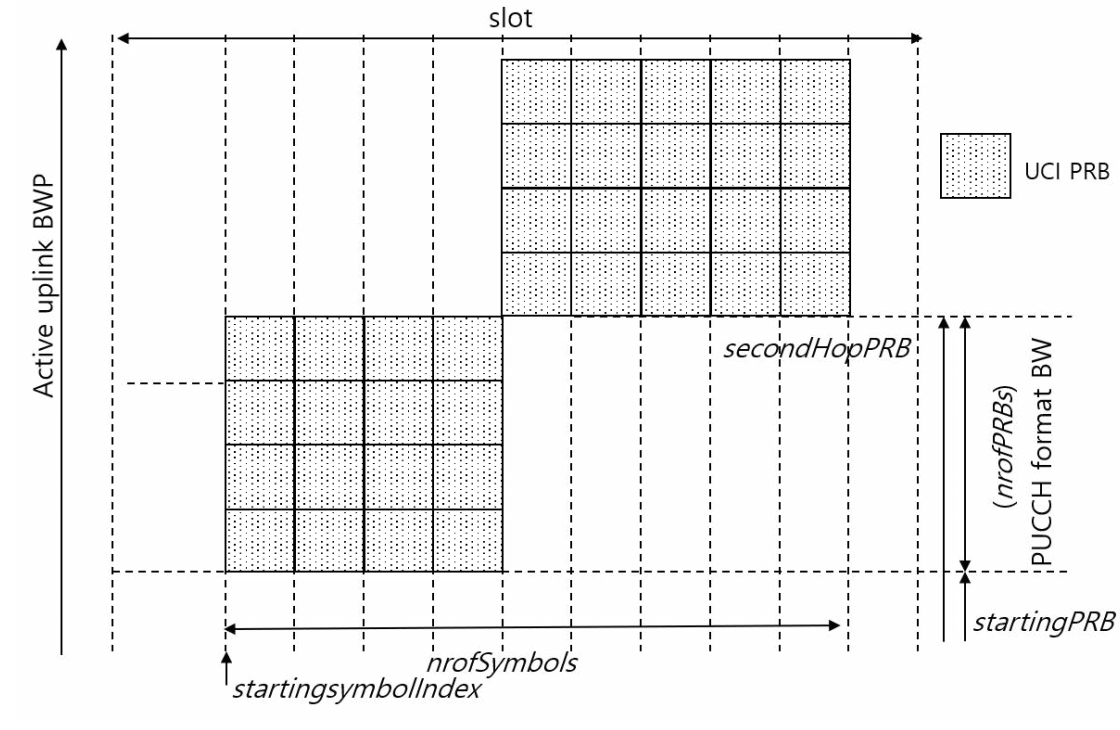
\includegraphics[scale=0.3 ]{RRC .png}
    \caption{ PUCCH resource allocation and related RRC parameters}
\end{figure}
\end{frame}

\begin{frame}{\textbf{System Description}}
\begin{figure}
    \centering
    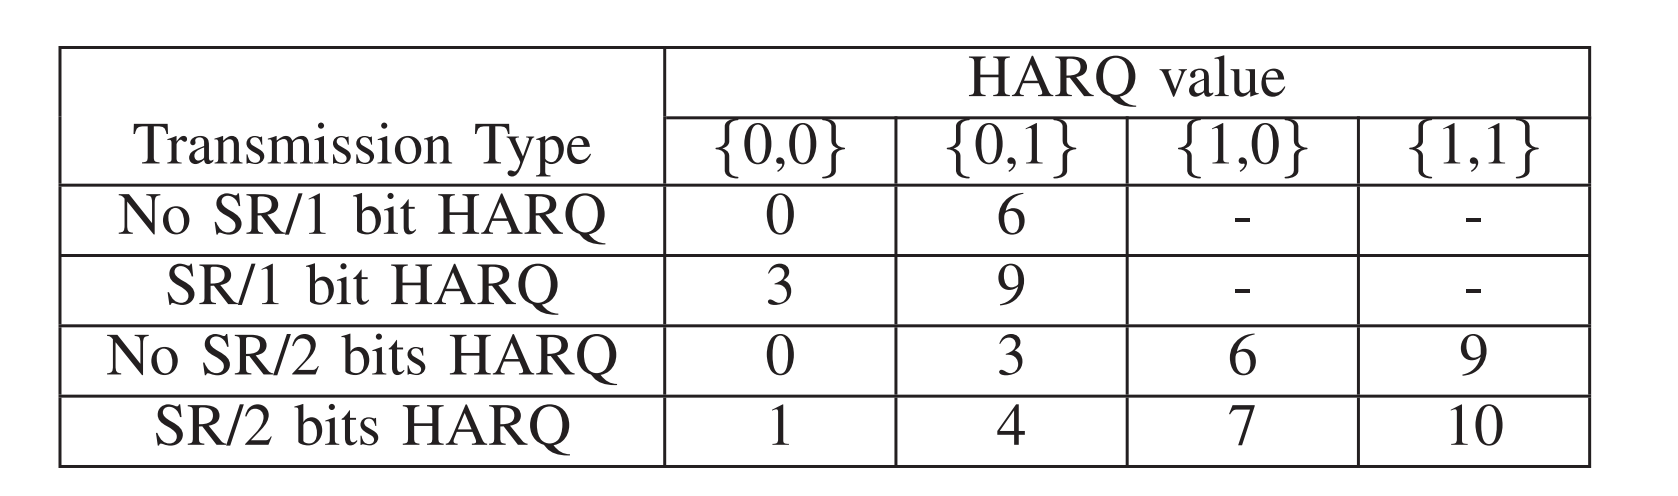
\includegraphics[scale=0.28 ]{MCS.png}
    \caption{$m_{CS}$ VALUE FOR HARQ/SR TRANSMISSION OF FORMAT 0}
\end{figure}
\end{frame}

\begin{frame}{\textbf{System description}}
\begin{itemize}
    \item . There are 4 possible different Low-PAPR sequences for one OFDM symbol transmission and 8 orthogonal candidates for two OFDM symbol transmission at the receiver side of gNB.
    \item  The received sequences are correlated with these sequences:
    \begin{align}
        C_{m}=\frac{1}{N_{r}}\sum_{r=0}^{N_{r}-1}\left| \frac{1}{N^{RB}_{sc}}\sum_{k=0}^{N^{RB}_{sc}-1}R_{r}(k)\times X_{m}^{*}(k)\right|
    \end{align}
\item $N_{r}$:no of RX branch.
\item  $R_{r}(k)$: received PUCCH sequence in the frequency domain
\item $ X_{m}^{*}(k)$:  conjugated sequence that m = $m_{CS}$
\item The demodulated UCI bits can be obtained by finding m that provides the maximum of $C_{m}$.
\end{itemize}
\end{frame}
   
\begin{frame}{\textbf{Performance Metrics}}
\begin{itemize}
    \item There are two performance metrics for NR PUCCH format 0.
\end{itemize}
\begin{block}{DTX to ACK probability}
It is the probability that ACK is detected when nothing was transmitted to gNB.
\begin{itemize}
\item Performance requirement: DTX to ACK probability $ < 1\%$
\end{itemize}
\end{block}
\begin{block}{Missed ACK probability}
 The  missed ACK probability is the probability of not detecting an ACK when an ACK was sent.
\begin{itemize}
\item Performance requirement: Missed ACK probability $ < 1\%$
\end{itemize}
\end{block}
\end{frame}
\begin{frame}{\textbf{TX and RX processing}}
    \begin{figure}
        \centering
        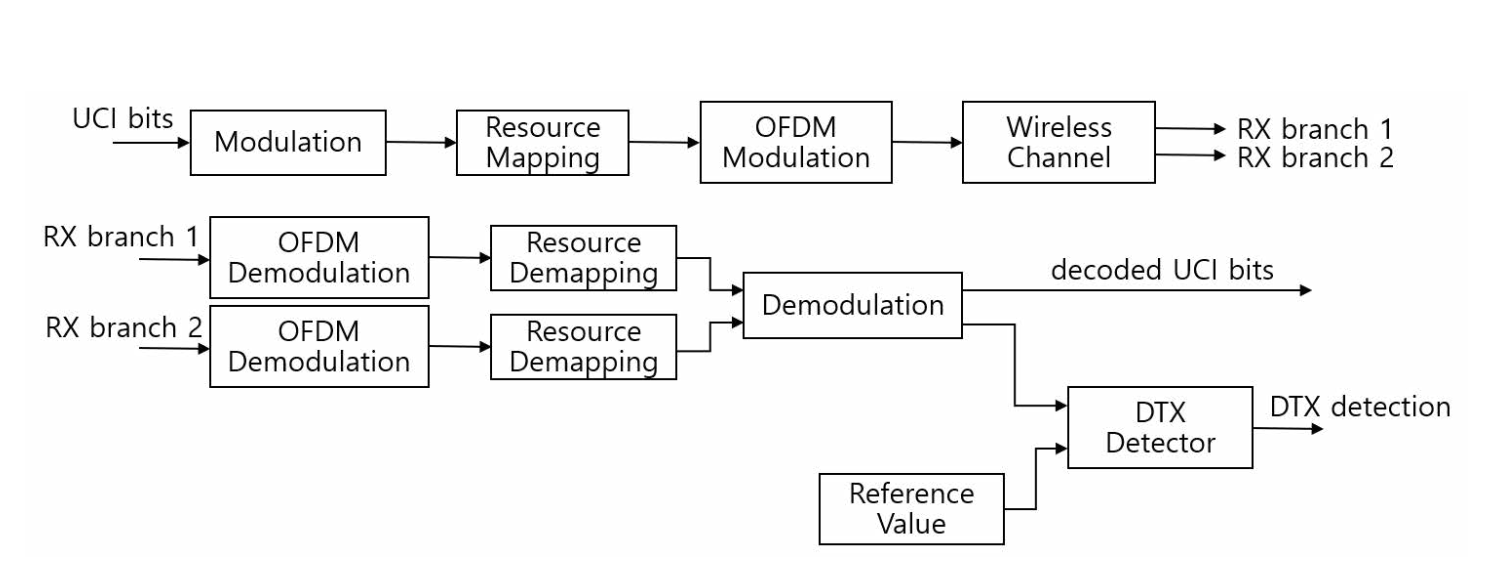
\includegraphics[scale=0.3]{TX_RX.png}
        \caption{TX and RX processing for PUCCH format 0}
       
    \end{figure}
\end{frame}
\begin{frame}{\textbf{Simulation results}}
\begin{itemize}
    \item In this section, two detection schemes of the DTX for PUCCH format 0 have been simulated.
    \item . In this link level simulation, DTX
threshold values for two detection algorithms are chosen to maintain at below 0.01 for DTX to ACK probability.
\item The performances
of two algorithms of alg0 (based on the power) and alg1 (based on the correlation) with 1 RX branch and 2 RX branch cases are compared.
\item  Both algorithms can get the
diversity gain, however the required SNR for the power based scheme does not meet the required SNR 3.8dB.
\item The reason for the better performance of the correlation based algorithm is due to the processing gain of the Low-PAPR sequence correlation under the fading channel.
\end{itemize}
    
\end{frame}
\begin{frame}{\textbf{Simulation results}}
\begin{figure}
    \centering
    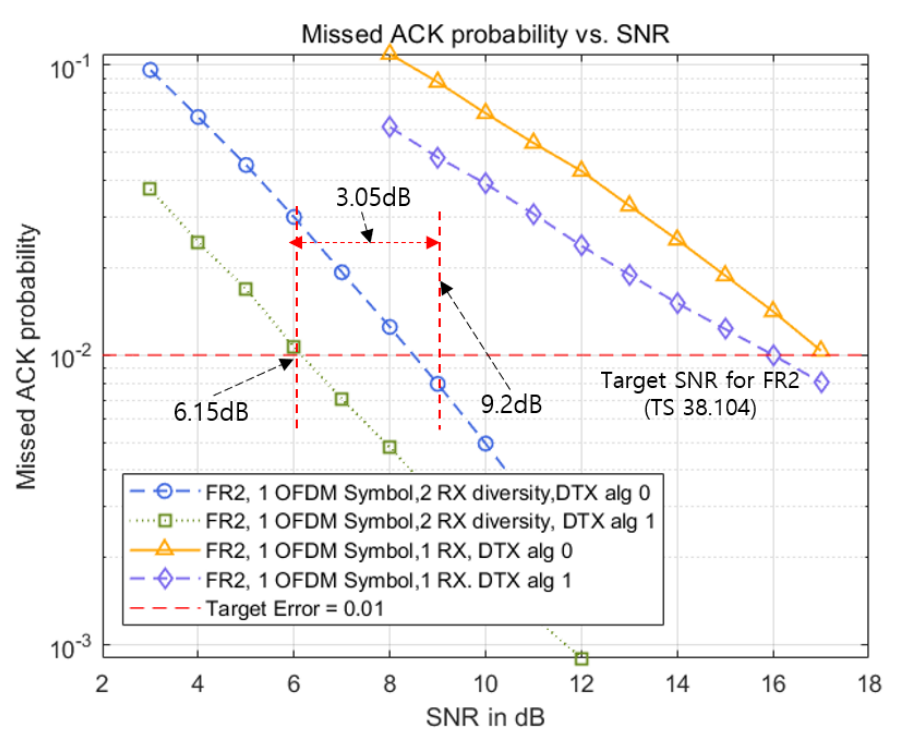
\includegraphics[scale=0.3]{OFDM1.png}
    \caption{ Missed ACK detection probability for 1 OFDM symbol}
\end{figure}
\end{frame}

\begin{frame}{\textbf{Simulation results}}
\begin{figure}
    \centering
    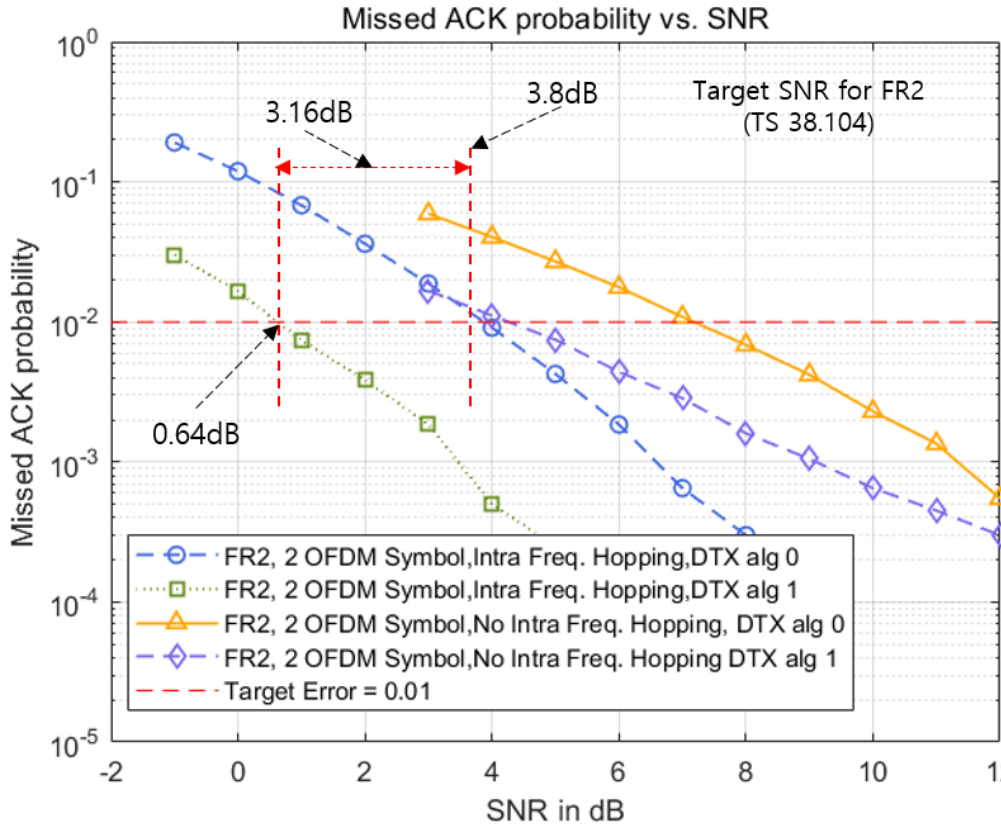
\includegraphics[scale=0.3]{OFDM2.png}
    \caption{Missed ACK detection probability for 2 OFDM symbol}
\end{figure}
\end{frame}

\begin{frame}{\textbf{Conclusion}}
\begin{itemize}
 \item The DTX is one of the most important functionality to save the battery life for a UE.
 \item The detection of DTX is essential at the receiver side of the gNB.
 \item Simulation results shows above two schemes for the 5G NR PUCCH format 0 satisfy the performance requirements.
 \item Two schemes are feasible and promising for the various deployments of 5G NR gNB such as the regular gNB, DU and IAB.
\end{itemize}
\end{frame}
\end{document}